% !TEX root = ../main.tex
\section{Regular Few-Shot Classification}
We include standard 5-way few-shot classification results in Table~\ref{tab:fewshot1_novel}. As
mentioned in the main text, a simple logistic regression model can achieve competitive performance
on few-shot classification using pretrained features. Our full model shows similar performance on
regular few-shot classification. This confirms that the learned regularizer is mainly solving the
interference problem between the base and novel classes.
\vspace{0.1in}

\begin{table}[h!]
\begin{small}
\begin{center}
\caption{Regular 5-way few-shot classification on \textit{mini-ImageNet}.
Note that this is purely few-shot, with no base classes. Applying logistic regression on pretrained
features achieves performance on-par with other competitive meta-learning approaches. * denotes our
own implementation.}
\label{tab:fewshot1_novel}
% \begin{minipage}[c]{0.5\textwidth}
% \hfill
% \resizebox{\columnwidth}{!}{
% \begin{tabular}{|c|c|c|c|}
\begin{tabular}{lccc}
% \hline
\toprule
Model        & Backbone & 1-shot                & 5-shot                \\
% \hline\hline 
\midrule                                                             
MatchingNets \citep{matching} 
             & C64      & 43.60                 & 55.30                 \\
Meta-LSTM \citep{metalstm} 
           & C32      & 43.40 $\pm$ 0.77      & 60.20 $\pm$ 0.71      \\
MAML \citep{maml}
             & C64      & 48.70 $\pm$ 1.84      & 63.10 $\pm$ 0.92      \\
RelationNet \citep{relationnet} 
             & C64      & 50.44 $\pm$ 0.82      & 65.32 $\pm$ 0.70      \\
R2-D2  \citep{diffsolver} 
           & C256     & 51.20 $\pm$ 0.60      & 68.20 $\pm$ 0.60      \\
SNAIL \citep{mishra2017meta} 
           & ResNet   & 55.71 $\pm$ 0.99      & 68.88 $\pm$ 0.92      \\
ProtoNet \citep{proto} 
             & C64      & 49.42 $\pm$ 0.78      & 68.20 $\pm$ 0.66      \\
ProtoNet*  \citep{proto} 
             & ResNet   & 50.09 $\pm$ 0.41      & 70.76 $\pm$ 0.19      \\
LwoF \citep{lwof} 
             & ResNet   & 55.45 $\pm$ 0.89      & \tb{70.92} $\pm$ 0.35 \\
% LwoF*        & ResNet   & \textbf{56.97} $\pm$ 0.24 & 70.50 $\pm$ 0.36 \\
% \hline
\midrule
LR           & ResNet   & 55.40 $\pm$ 0.51      & 70.17 $\pm$ 0.46 \\
% LR +S        & ResNet   & 55.06 $\pm$ 0.52      & 70.32 $\pm$ 0.46 \\
Ours Full     & ResNet   & \tb{55.75} $\pm$ 0.51 & 70.14 $\pm$ 0.44 \\
% \hline
\bottomrule
\end{tabular}
% }
% \end{minipage}
\end{center}
\end{small}
\end{table}

\section{Visualization of Few-Shot Episodes}
We include more visualization of few-shot episodes in Figure~\ref{fig:moreviz}, highlighting the differences between our method and ``Dynamic Few-Shot Learning without Forgetting''~\citep{lwof}.
\begin{figure}[h!]
\centering
\iflatexml
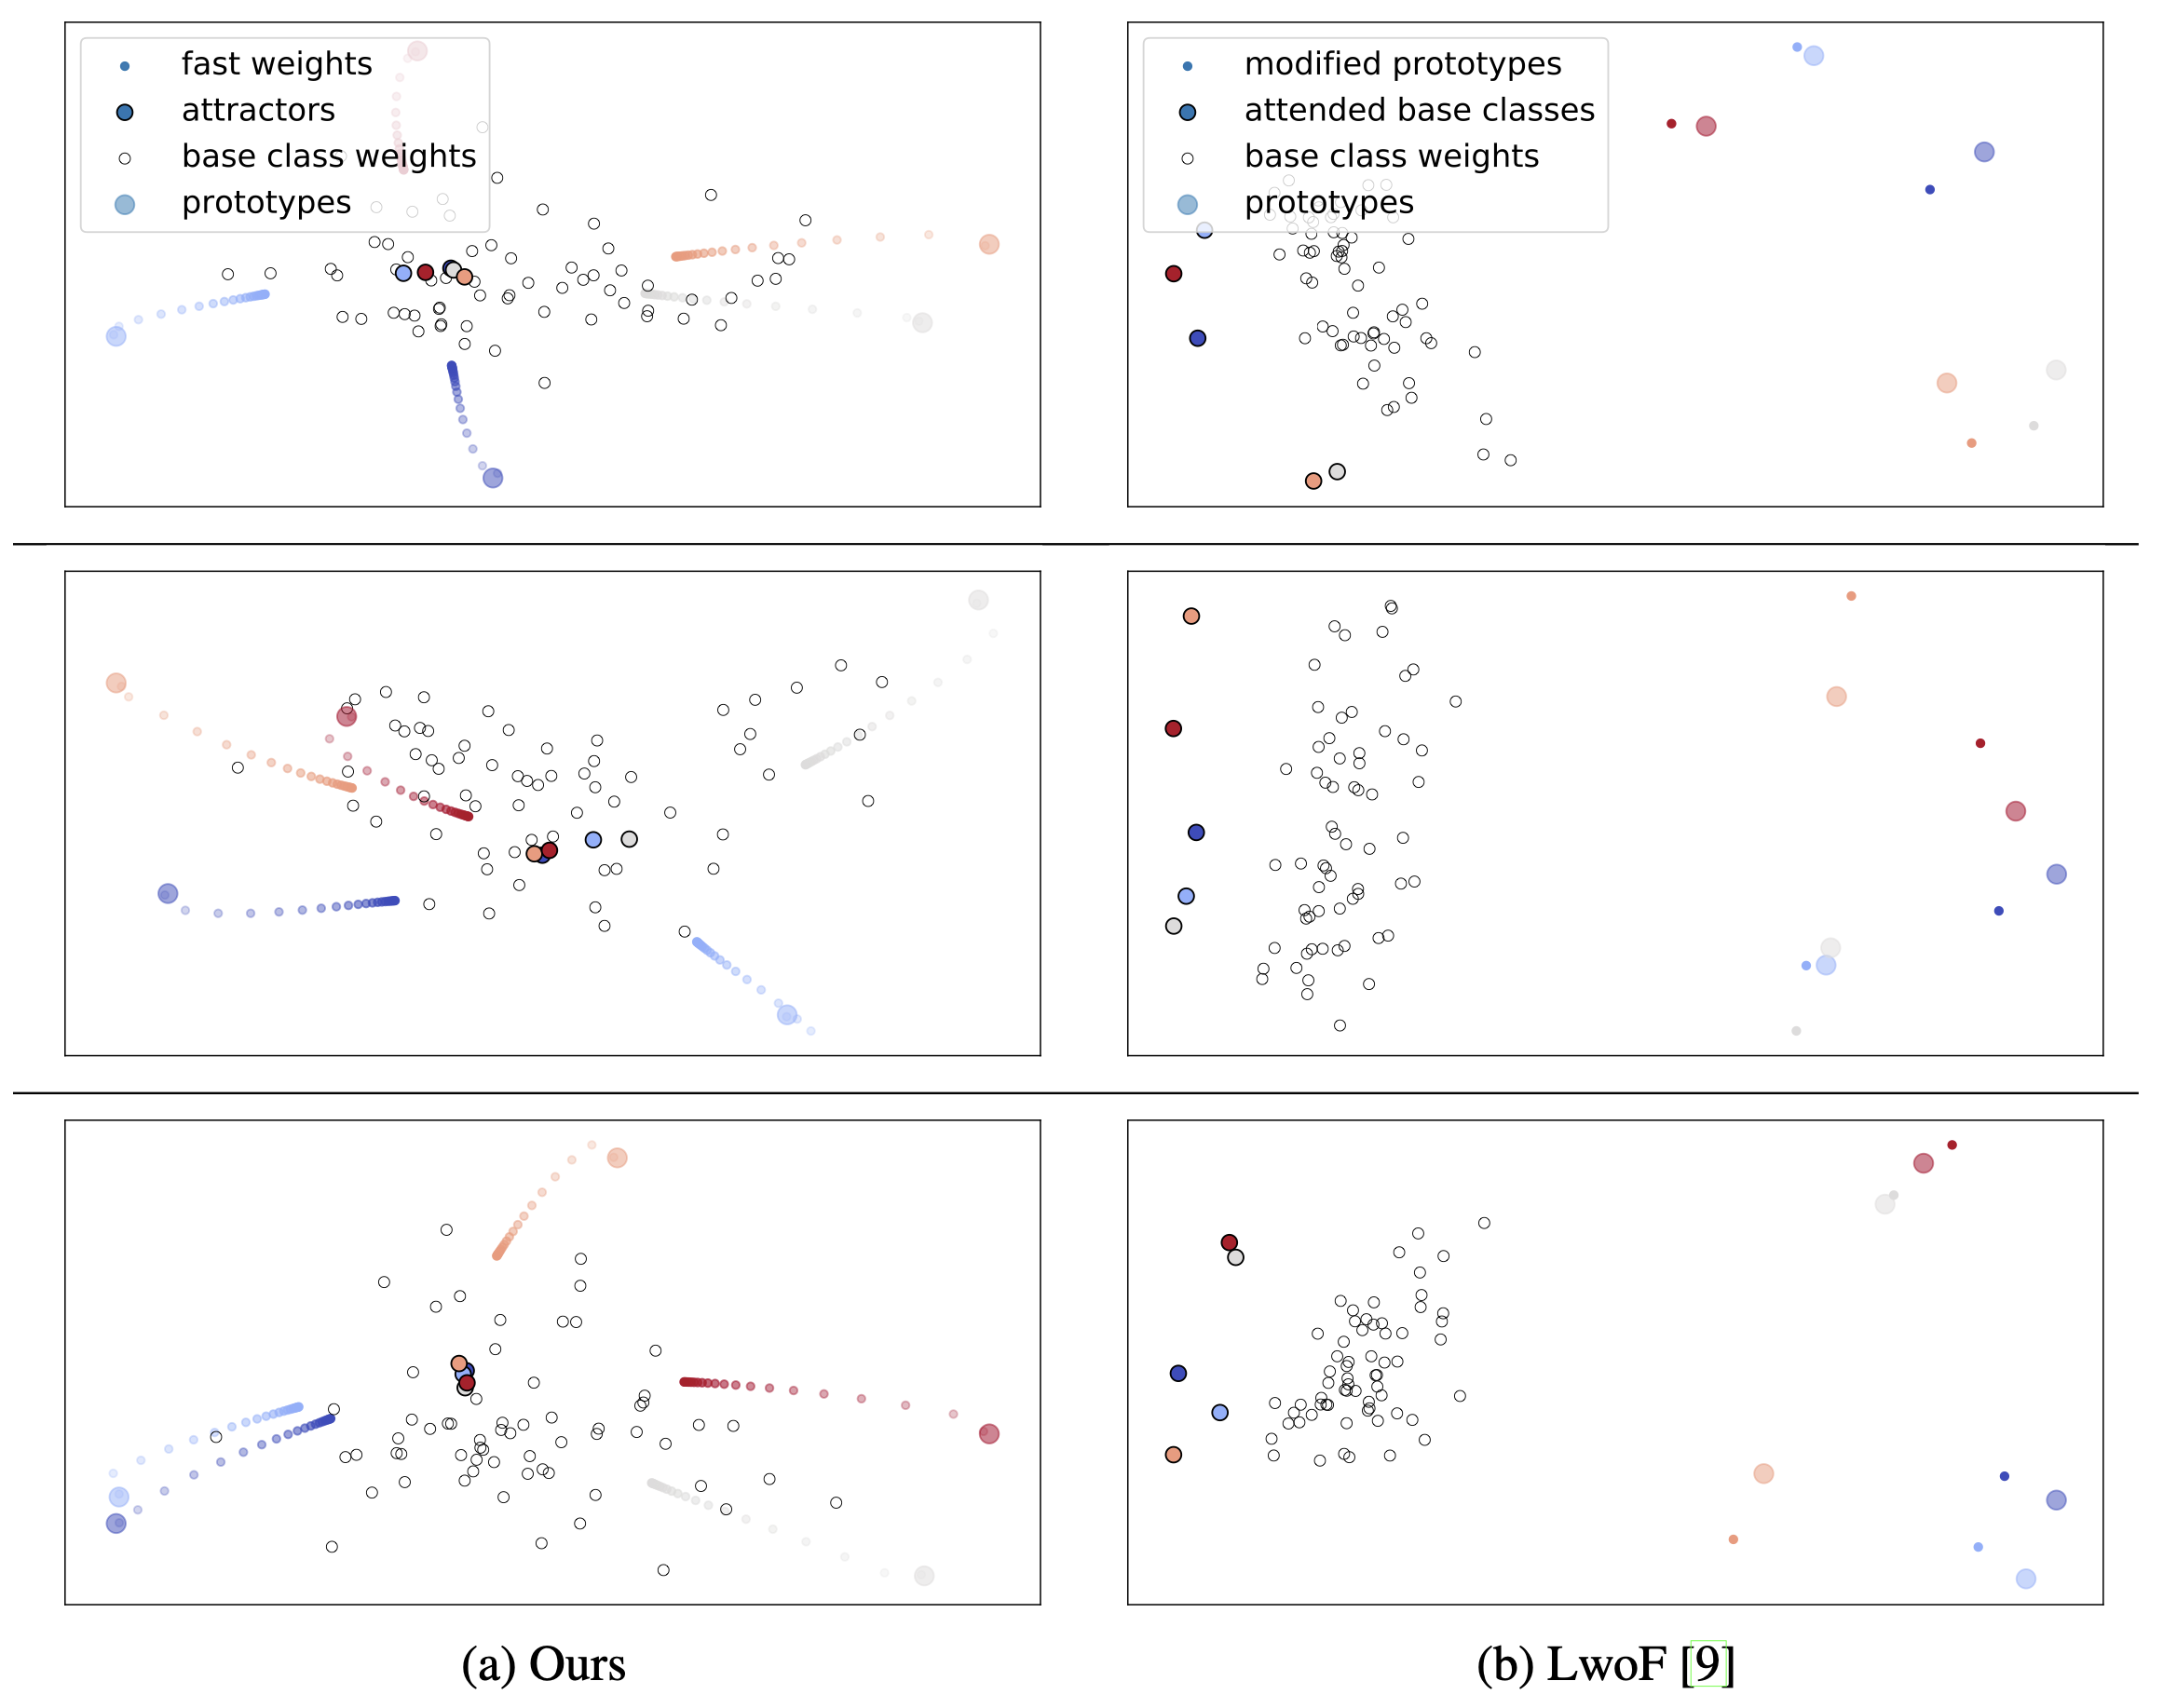
\includegraphics[width=6\textwidth]{figures/attractor_progress_app.png}
\else
\begin{minipage}[c]{\textwidth}
\begin{small}
\begin{tabular}{cc}
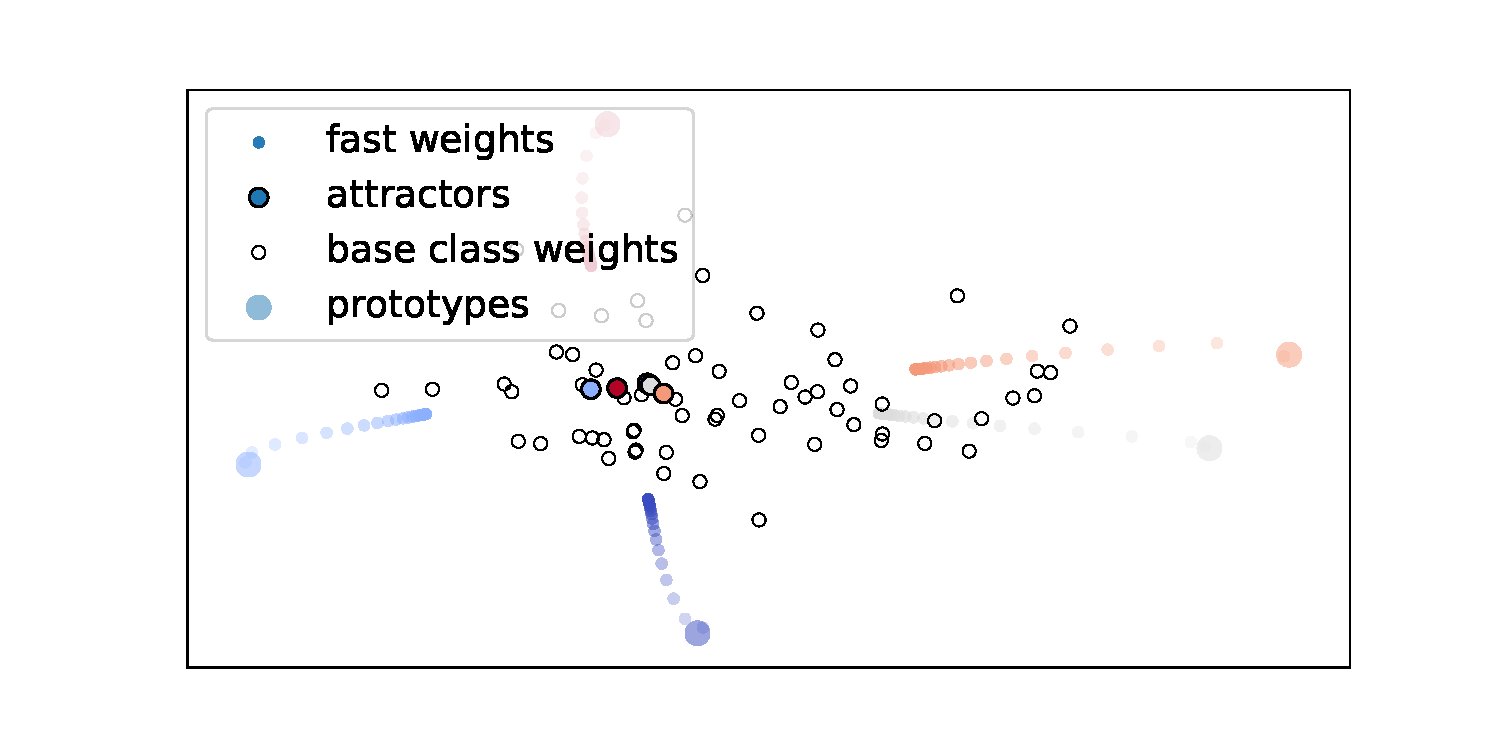
\includegraphics[width=0.45\textwidth,trim={2.8cm 1cm 2.5cm 1cm},clip]{figures/attractor_progress_0.pdf} & 
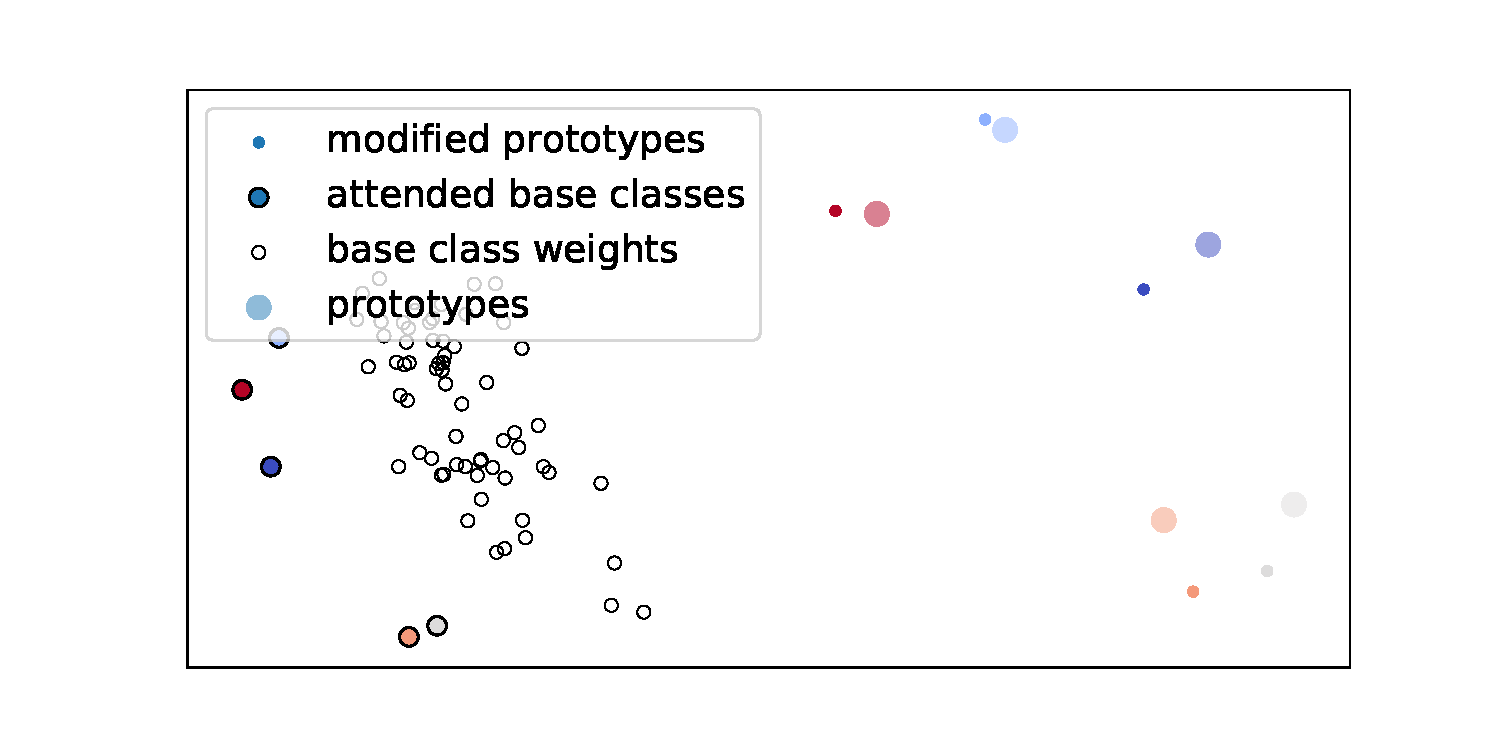
\includegraphics[width=0.45\textwidth,trim={2.8cm 1cm 2.5cm 1cm},clip]{figures/lwof_progress_0.pdf}\\
\hline
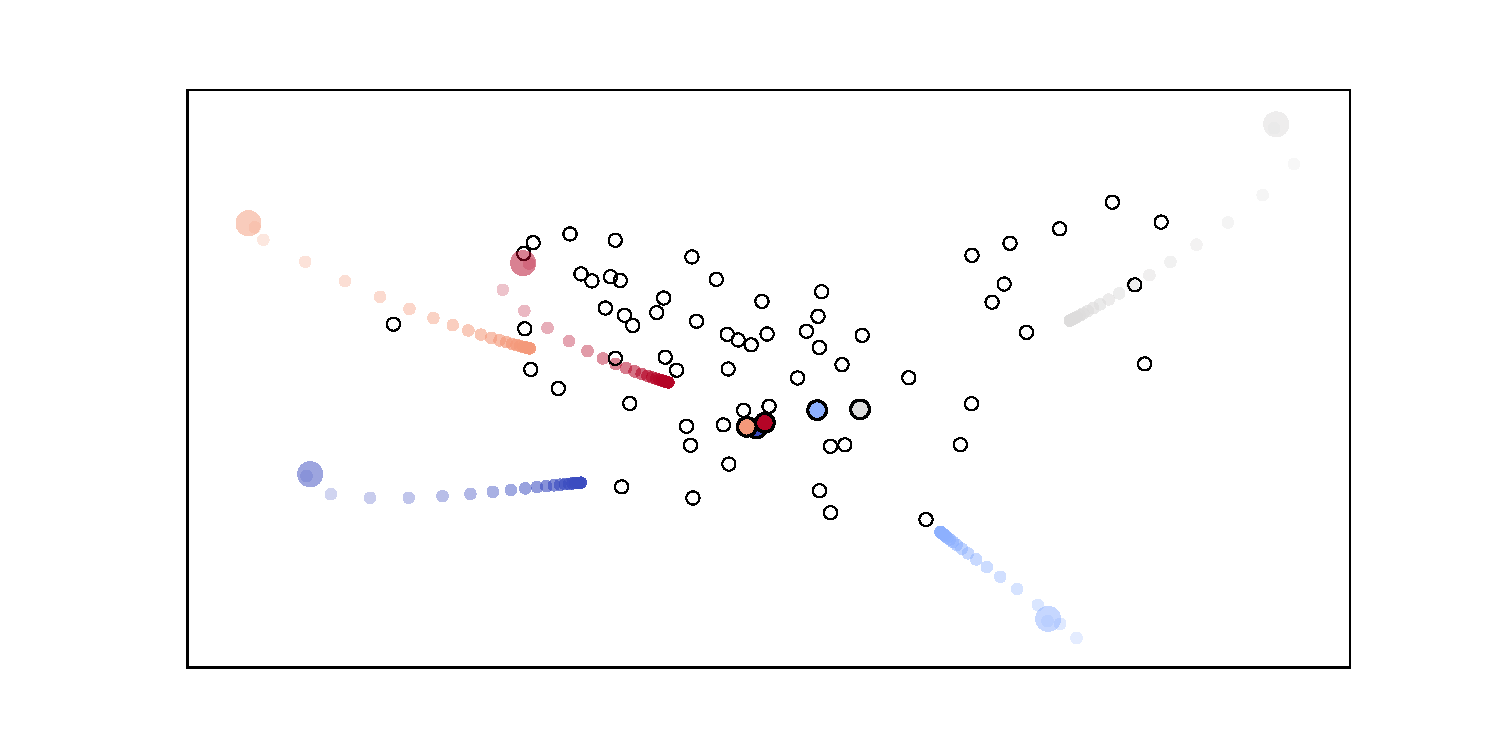
\includegraphics[width=0.45\textwidth,trim={2.8cm 1cm 2.5cm 1cm},clip]{figures/attractor_progress_3_noleg.pdf} & 
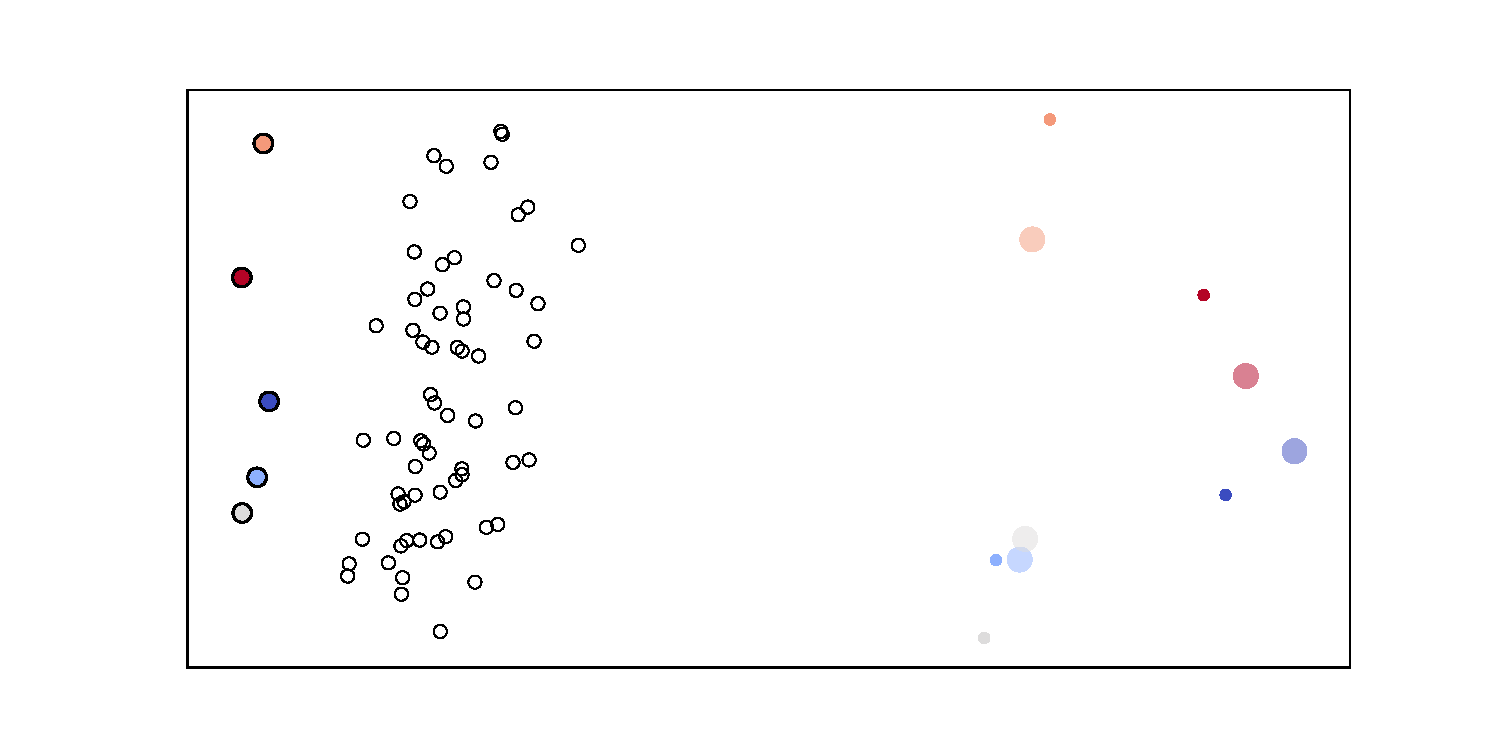
\includegraphics[width=0.45\textwidth,trim={2.8cm 1cm 2.5cm 1cm},clip]{figures/lwof_progress_3_noleg.pdf}\\
\hline
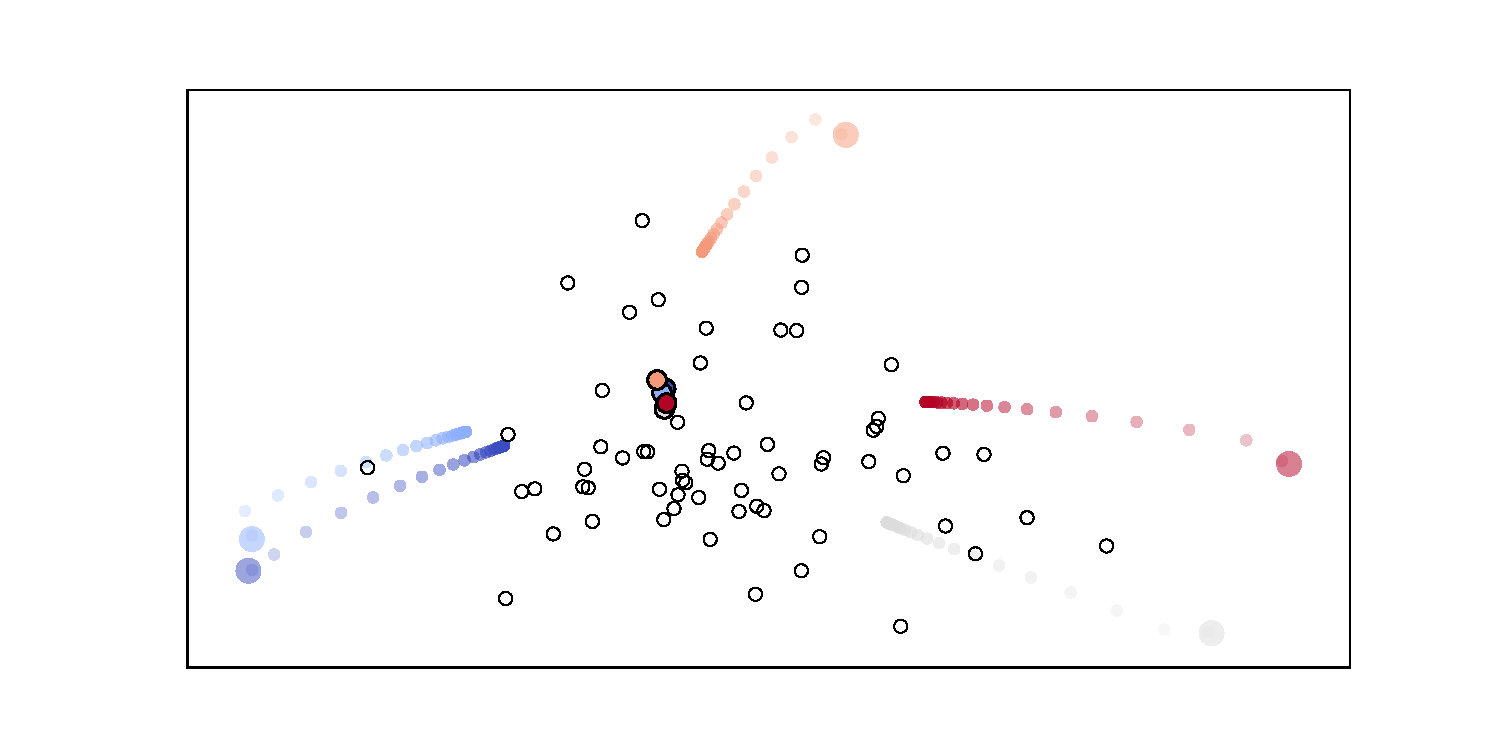
\includegraphics[width=0.45\textwidth,trim={2.8cm 1cm 2.5cm 1cm},clip]{figures/attractor_progress_8_noleg.pdf} & 
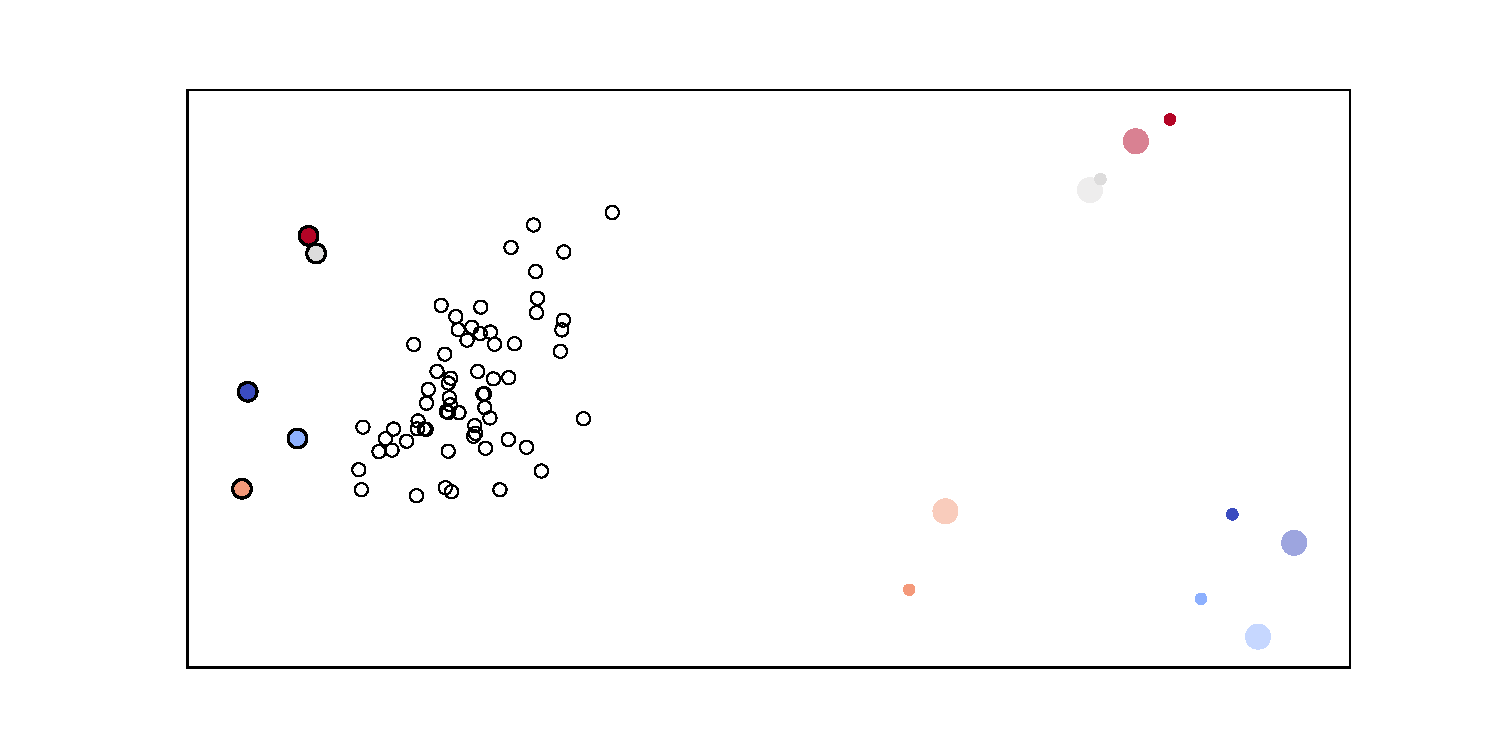
\includegraphics[width=0.45\textwidth,trim={2.8cm 1cm 2.5cm 1cm},clip]{figures/lwof_progress_8_noleg.pdf}\\
(a) Ours & (b) LwoF \citep{lwof}
\end{tabular}
\end{small}
\end{minipage}
\fi
\caption{Visualization of 5-shot 64+5-way episodes on \textit{mini}-ImageNet using PCA.}
\label{fig:moreviz}
\end{figure}

\section{Visualization of Attention Attractors}
To further understand the attractor mechanism, we picked 5 semantic classes in
\textit{mini}-ImageNet and visualized their the attention attractors across 20 episodes, shown in
Figure~\ref{fig:attractorviz}. The attractors roughly form semantic clusters, whereas the static
attractor stays in the center of all attractors.
% !TEX root = ../supp.tex
\begin{figure}[h!]
\centering
\iflatexml
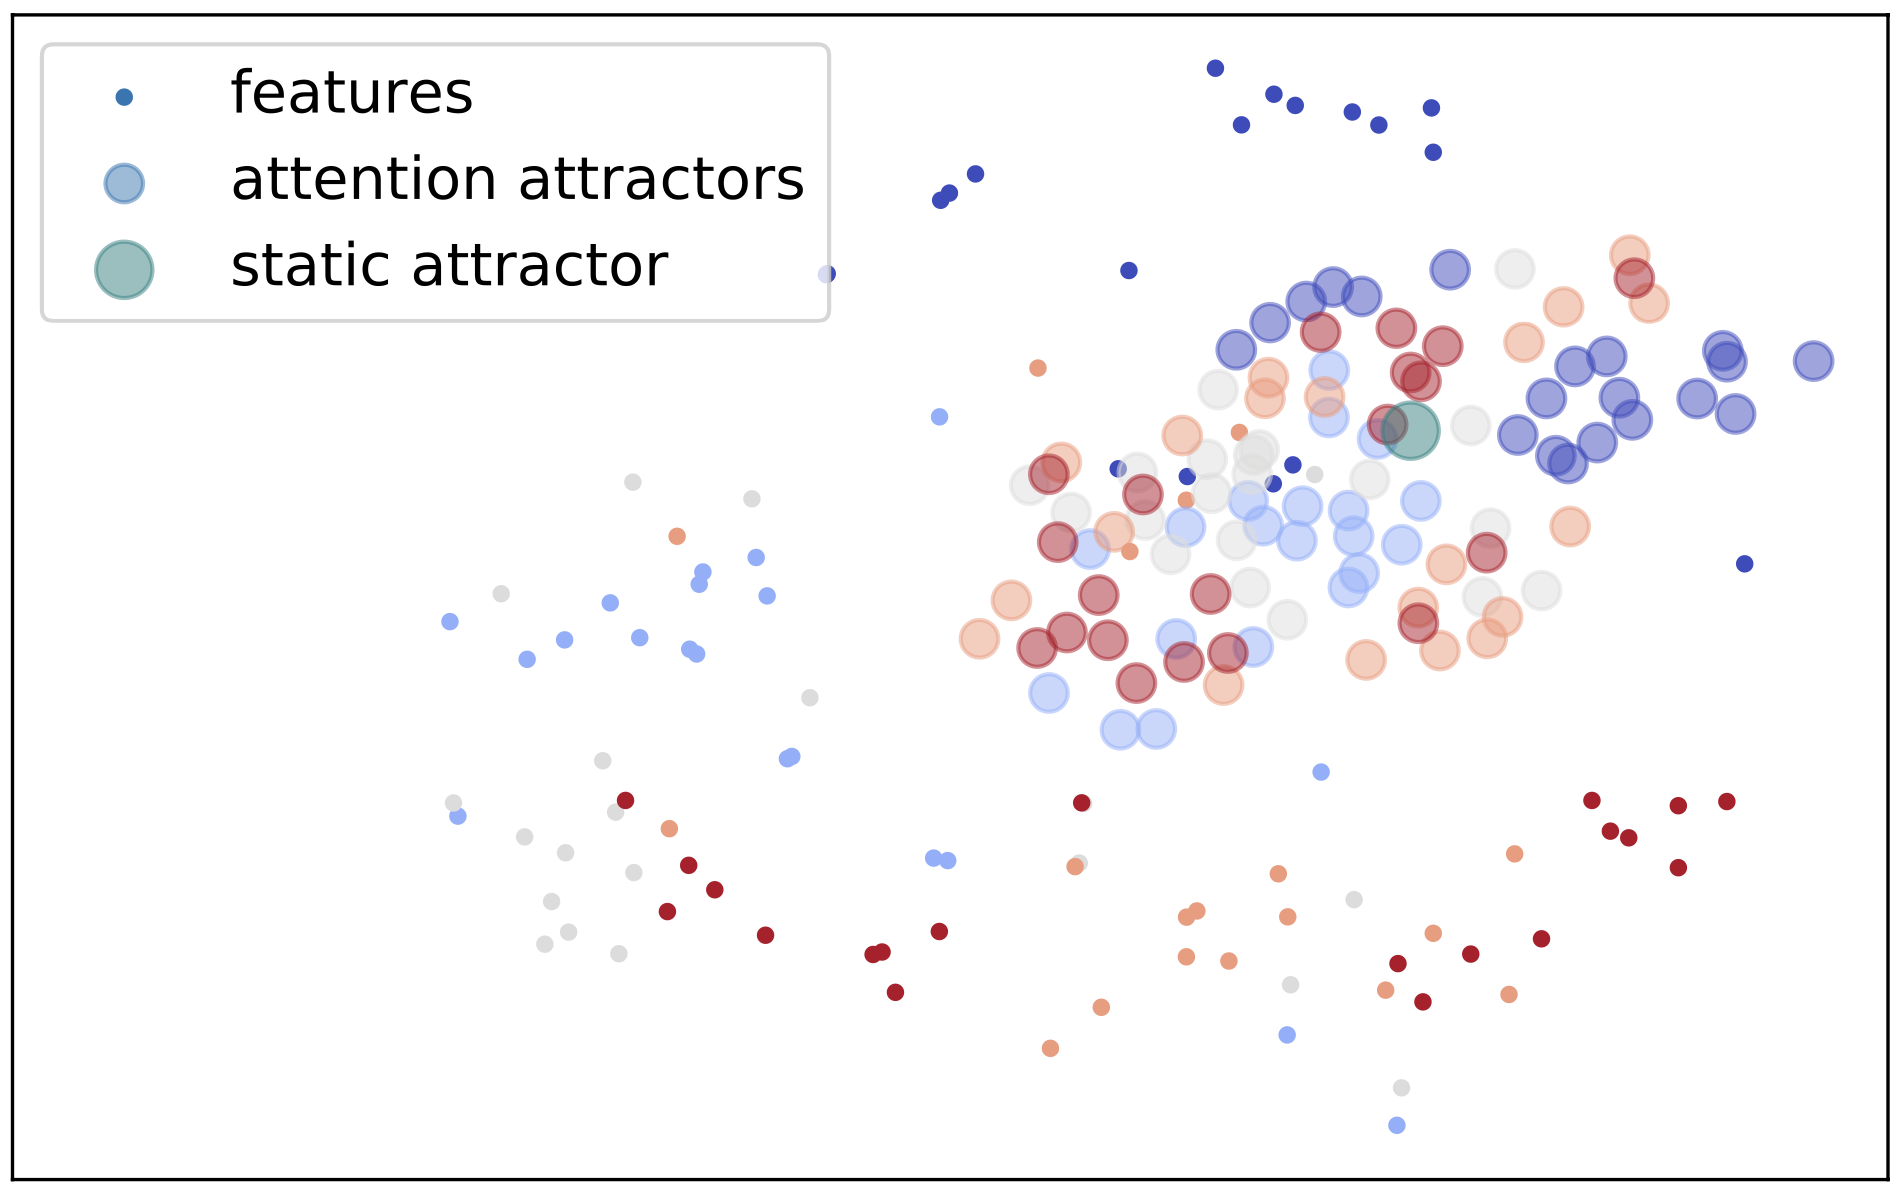
\includegraphics[width=4\textwidth]{figures/attractor_tsne.png}
\else
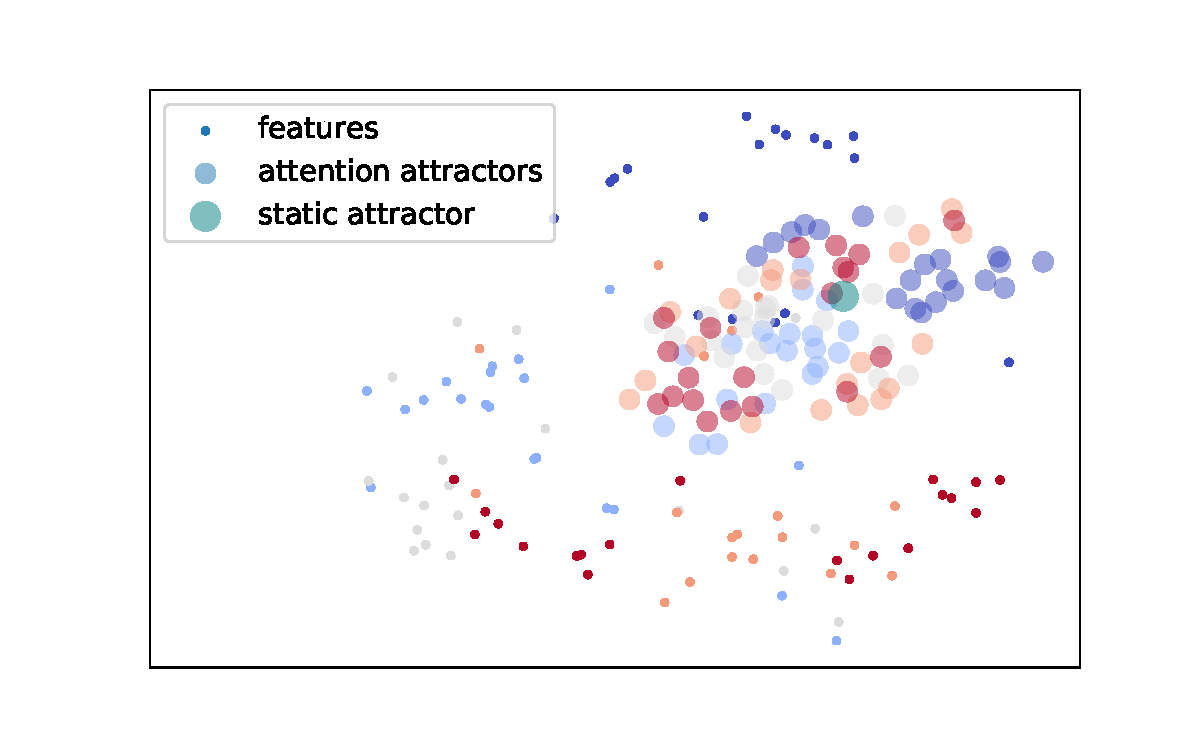
\includegraphics[width=0.6\textwidth,trim={1cm 0.5cm 1.6cm 1cm},clip]{figures/attractor_tsne.pdf}
\fi
\caption{Visualization of example features and attractors using t-SNE. This plot shows a 5-way
5-shot episode on \textit{mini}-ImageNet. 512-dimensional feature vectors and attractor vectors
are projected to a 2-dim space. Color represents the label class of the example. The static
attractor (\textcolor{teal}{teal}) appears at the center of the attention attractors, which roughly
form clusters based on the classes.}
\label{fig:attractorviz}
\end{figure}


\begin{table}
\centering
\caption{Full ablation results on 64+5-way {\it mini}-ImageNet}
\iflatexml
% \resizebox{0.8\textwidth}{!}{
\begin{tabular}{c|cccc|cccc}
\toprule
          & \multicolumn{4}{c|}{1-shot}           & \multicolumn{4}{c}{5-shot} \\
          & Acc. $\ua$            & \D         & \Da    &\Db     & Acc. $\ua$            & \D         & \Da    & \Db     \\
\midrule                                                                                                                
LR        & 52.74 $\pm$ 0.24      & -13.95     & -8.98  & -24.32 & 60.34 $\pm$ 0.20      & -13.60     & -10.81 & -15.97  \\
LR +S     & 53.63 $\pm$ 0.30      & -12.53     & -9.44  & -15.62 & 62.50 $\pm$ 0.30      & -11.29     & -13.84 & -8.75   \\
LR +A     & \tb{55.31} $\pm$ 0.32 & \tb{-11.72}& -12.72 & -10.71  & 63.00 $\pm$ 0.29      & -10.80     & -13.59 & -8.01   \\
\midrule                                                                                                                             
MLP       & 49.36 $\pm$ 0.29      & -16.78     & -8.95  & -24.61 & 60.85 $\pm$ 0.29      & -12.62     & -11.35 & -13.89  \\
MLP +S    & 54.46 $\pm$ 0.31      & -11.74     & -12.73 & -10.74 & 62.79 $\pm$ 0.31      & -10.77     & -12.61 & -8.80   \\
MLP +A    & 54.95 $\pm$ 0.30      & -11.84     & -12.81 & -10.87 & \tb{63.04} $\pm$ 0.30 & \tb{-10.66}& -12.55 & -8.77   \\
\bottomrule
\end{tabular}
% }
\else
\resizebox{0.8\textwidth}{!}{
\begin{tabular}{c|cccc|cccc}
\toprule
          & \multicolumn{4}{c|}{1-shot}           & \multicolumn{4}{c}{5-shot} \\
          & Acc. $\ua$            & \D         & \Da    &\Db     & Acc. $\ua$            & \D         & \Da    & \Db     \\
\midrule                                                                                                                
LR        & 52.74 $\pm$ 0.24      & -13.95     & -8.98  & -24.32 & 60.34 $\pm$ 0.20      & -13.60     & -10.81 & -15.97  \\
LR +S     & 53.63 $\pm$ 0.30      & -12.53     & -9.44  & -15.62 & 62.50 $\pm$ 0.30      & -11.29     & -13.84 & -8.75   \\
LR +A     & \tb{55.31} $\pm$ 0.32 & \tb{-11.72}& -12.72 & -10.71  & 63.00 $\pm$ 0.29      & -10.80     & -13.59 & -8.01   \\
\midrule                                                                                                                             
MLP       & 49.36 $\pm$ 0.29      & -16.78     & -8.95  & -24.61 & 60.85 $\pm$ 0.29      & -12.62     & -11.35 & -13.89  \\
MLP +S    & 54.46 $\pm$ 0.31      & -11.74     & -12.73 & -10.74 & 62.79 $\pm$ 0.31      & -10.77     & -12.61 & -8.80   \\
MLP +A    & 54.95 $\pm$ 0.30      & -11.84     & -12.81 & -10.87 & \tb{63.04} $\pm$ 0.30 & \tb{-10.66}& -12.55 & -8.77   \\
\bottomrule
\end{tabular}
}
\fi
\end{table}

\begin{table*}[t!]
\centering
\caption{Full ablation results on 200+5-way {\it tiered}-ImageNet}
\iflatexml
\begin{tabular}{c|cccc|cccc}
\toprule
          & \multicolumn{4}{c|}{1-shot}           & \multicolumn{4}{c}{5-shot} \\
          & Acc. $\ua$            & \D         & \Da    & \Db    & Acc. $\ua$            & \D         & \Da    & \Db     \\
\midrule                                                                                                              
LR        & 48.84 $\pm$ 0.23      & -10.44     & -11.65 & -9.24  & 62.08 $\pm$ 0.20      & -8.00      & -5.49  & -10.51  \\
LR +S     & 55.36 $\pm$ 0.32      & -6.88      & -7.21  & -6.55  & 65.53 $\pm$ 0.30      & -4.68      & -4.72  & -4.63   \\
LR +A     & 55.98 $\pm$ 0.32      & \tb{-6.07} & -6.64  & -5.51  & 65.58 $\pm$ 0.29      & \tb{-4.39} & -4.87  & -3.91   \\
\midrule                                                                                                                                           
MLP       & 41.22 $\pm$ 0.35      & -10.61     & -11.25 & -9.98  & 62.70 $\pm$ 0.31      & -7.44      & -6.05  & -8.82   \\
MLP +S    & \tb{56.16} $\pm$ 0.32 & -6.28      & -6.83  & -5.73  & \tb{65.80} $\pm$ 0.31 & -4.58      & -4.66  & -4.51   \\
MLP +A    & 56.11 $\pm$ 0.33      & 6.11       & -6.79  & -5.43  & 65.52 $\pm$ 0.31      & -4.48      & -4.91  & -4.05   \\
\bottomrule
\end{tabular}
\else
\resizebox{0.8\textwidth}{!}{
\begin{tabular}{c|cccc|cccc}
\toprule
          & \multicolumn{4}{c|}{1-shot}           & \multicolumn{4}{c}{5-shot} \\
          & Acc. $\ua$            & \D         & \Da    & \Db    & Acc. $\ua$            & \D         & \Da    & \Db     \\
\midrule                                                                                                              
LR        & 48.84 $\pm$ 0.23      & -10.44     & -11.65 & -9.24  & 62.08 $\pm$ 0.20      & -8.00      & -5.49  & -10.51  \\
LR +S     & 55.36 $\pm$ 0.32      & -6.88      & -7.21  & -6.55  & 65.53 $\pm$ 0.30      & -4.68      & -4.72  & -4.63   \\
LR +A     & 55.98 $\pm$ 0.32      & \tb{-6.07} & -6.64  & -5.51  & 65.58 $\pm$ 0.29      & \tb{-4.39} & -4.87  & -3.91   \\
\midrule                                                                                                                                           
MLP       & 41.22 $\pm$ 0.35      & -10.61     & -11.25 & -9.98  & 62.70 $\pm$ 0.31      & -7.44      & -6.05  & -8.82   \\
MLP +S    & \tb{56.16} $\pm$ 0.32 & -6.28      & -6.83  & -5.73  & \tb{65.80} $\pm$ 0.31 & -4.58      & -4.66  & -4.51   \\
MLP +A    & 56.11 $\pm$ 0.33      & 6.11       & -6.79  & -5.43  & 65.52 $\pm$ 0.31      & -4.48      & -4.91  & -4.05   \\
\bottomrule
\end{tabular}
}
\fi
\end{table*}

\section{Dataset Statistics}
In this section, we include more details on the datasets we used in our experiments.
% We include the dataset statistics in Table~\ref{tab:stats}. In \textit{mini}-ImageNet, we use the
% training set for both pretraining and meta-learning. For testing base class classification
% performance, we included the same val/test set as \citep{lwof}. Since the meta-training set is same
% as meta-learning, in each training episode, we masked out the 5 base classes in the base classifier,
% to ``pretend'' they are few-shot classes. In \textit{tiered}-ImageNet, we splits the original
% training set, Train-A and Train-B, for pretraining and meta-learning respectively.

\begin{table}[h]
\begin{small}
\caption{\textit{mini}-ImageNet and \textit{tiered}-ImageNet split statistics}
\vspace{-0.1in}
\label{tab:stats}
\begin{center}
\begin{tabular}{cc|crr|crr}
\toprule
&& \multicolumn{3}{c|}{\textit{mini}-ImageNet}& \multicolumn{3}{c}{\textit{tiered}-ImageNet} \\
Classes                & Purpose & Split         & N. Cls  & N. Img  & Split           & N. Cls   & N. Img \\
\midrule
\multirow{3}{*}{Base}  & Train   & Train-Train   & 64      & 38,400  & Train-A-Train   & 200      & 203,751   \\
                      & Val     & Train-Val     & 64      & 18,748  & Train-A-Val     & 200      & 25,460    \\
                      & Test    & Train-Test    & 64      & 19,200  & Train-A-Test    & 200      & 25,488    \\
\midrule
\multirow{3}{*}{Novel} & Train   & Train-Train   & 64      & 38,400  & Train-B         & 151      & 193,996   \\
                      & Val     & Val           & 16      & 9,600   & Val             & 97       & 124,261   \\
                      & Test    & Test          & 20      & 12,000  & Test            & 160      & 206,209   \\
\bottomrule
\end{tabular}
\end{center}
\end{small}
\vspace{-0.2in}
\end{table}

\subsection{Validation and testing splits for base classes}
In standard few-shot learning, meta-training, validation, and test set have disjoint sets of object
classes. However, in our incremental few-shot learning setting, to evaluate the model performance on
the base class predictions, additional splits of validation and test splits of the meta-training set
are required. Splits and dataset statistics are listed in Table~\ref{tab:stats}. For
\textit{mini}-ImageNet, \citet{lwof} released additional images for evaluating training set, namely
``Train-Val'' and ``Train-Test''. For \textit{tiered}-ImageNet, we split out $\approx$ 20\% of the
images for validation and testing of the base classes.

\subsection{Novel classes}
In \textit{mini}-ImageNet experiments, the same training set is used for both $\mathcal{D}_a$ and
$\mathcal{D}_b$. In order to pretend that the classes in the few-shot episode are novel, following
\citet{lwof}, we masked the base classes in $W_a$, which contains 64 base classes. In other words, we
essentially train for a 59+5 classification task. We found that under this setting, the progress
of meta-learning in the second stage is not very significant, since all classes have already been
seen before.

In \textit{tiered}-ImageNet experiments, to emulate the process of learning novel classes during the
second stage, we split the training classes into base classes (``Train-A'') with 200 classes and novel classes (``Train-B'') with 151 classes, just for meta-learning purpose.
During the first stage the classifier is trained using Train-A-Train data. In each meta-learning episode we sample few-shot examples from the novel classes (Train-B) and a query base set from Train-A-Val.  

{\bf 200 Base Classes (``Train-A''):}

{\tt n02128757, n02950826, n01694178, n01582220, n03075370, n01531178, n03947888, n03884397, n02883205, n03788195, n04141975, n02992529, n03954731, n03661043, n04606251, n03344393, n01847000, n03032252, n02128385, n04443257, n03394916, n01592084, n02398521, n01748264, n04355338, n02481823, n03146219, n02963159, n02123597, n01675722, n03637318, n04136333, n02002556, n02408429, n02415577, n02787622, n04008634, n02091831, n02488702, n04515003, n04370456, n02093256, n01693334, n02088466, n03495258, n02865351, n01688243, n02093428, n02410509, n02487347, n03249569, n03866082, n04479046, n02093754, n01687978, n04350905, n02488291, n02804610, n02094433, n03481172, n01689811, n04423845, n03476684, n04536866, n01751748, n02028035, n03770439, n04417672, n02988304, n03673027, n02492660, n03840681, n02011460, n03272010, n02089078, n03109150, n03424325, n02002724, n03857828, n02007558, n02096051, n01601694, n04273569, n02018207, n01756291, n04208210, n03447447, n02091467, n02089867, n02089973, n03777754, n04392985, n02125311, n02676566, n02092002, n02051845, n04153751, n02097209, n04376876, n02097298, n04371430, n03461385, n04540053, n04552348, n02097047, n02494079, n03457902, n02403003, n03781244, n02895154, n02422699, n04254680, n02672831, n02483362, n02690373, n02092339, n02879718, n02776631, n04141076, n03710721, n03658185, n01728920, n02009229, n03929855, n03721384, n03773504, n03649909, n04523525, n02088632, n04347754, n02058221, n02091635, n02094258, n01695060, n02486410, n03017168, n02910353, n03594734, n02095570, n03706229, n02791270, n02127052, n02009912, n03467068, n02094114, n03782006, n01558993, n03841143, n02825657, n03110669, n03877845, n02128925, n02091032, n03595614, n01735189, n04081281, n04328186, n03494278, n02841315, n03854065, n03498962, n04141327, n02951585, n02397096, n02123045, n02095889, n01532829, n02981792, n02097130, n04317175, n04311174, n03372029, n04229816, n02802426, n03980874, n02486261, n02006656, n02025239, n03967562, n03089624, n02129165, n01753488, n02124075, n02500267, n03544143, n02687172, n02391049, n02412080, n04118776, n03838899, n01580077, n04589890, n03188531, n03874599, n02843684, n02489166, n01855672, n04483307, n02096177, n02088364.}

{\bf 151 Novel Classes (``Train-B''):}

{\tt n03720891, n02090379, n03134739, n03584254, n02859443, n03617480, n01677366, n02490219, n02749479, n04044716, n03942813, n02692877, n01534433, n02708093, n03804744, n04162706, n04590129, n04356056, n01729322, n02091134, n03788365, n01739381, n02727426, n02396427, n03527444, n01682714, n03630383, n04591157, n02871525, n02096585, n02093991, n02013706, n04200800, n04090263, n02493793, n03529860, n02088238, n02992211, n03657121, n02492035, n03662601, n04127249, n03197337, n02056570, n04005630, n01537544, n02422106, n02130308, n03187595, n03028079, n02098413, n02098105, n02480855, n02437616, n02123159, n03803284, n02090622, n02012849, n01744401, n06785654, n04192698, n02027492, n02129604, n02090721, n02395406, n02794156, n01860187, n01740131, n02097658, n03220513, n04462240, n01737021, n04346328, n04487394, n03627232, n04023962, n03598930, n03000247, n04009552, n02123394, n01729977, n02037110, n01734418, n02417914, n02979186, n01530575, n03534580, n03447721, n04118538, n02951358, n01749939, n02033041, n04548280, n01755581, n03208938, n04154565, n02927161, n02484975, n03445777, n02840245, n02837789, n02437312, n04266014, n03347037, n04612504, n02497673, n03085013, n02098286, n03692522, n04147183, n01728572, n02483708, n04435653, n02480495, n01742172, n03452741, n03956157, n02667093, n04409515, n02096437, n01685808, n02799071, n02095314, n04325704, n02793495, n03891332, n02782093, n02018795, n03041632, n02097474, n03404251, n01560419, n02093647, n03196217, n03325584, n02493509, n04507155, n03970156, n02088094, n01692333, n01855032, n02017213, n02423022, n03095699, n04086273, n02096294, n03902125, n02892767, n02091244, n02093859, n02389026.}
